\documentclass{article}
\usepackage{tikz}
\usepackage{amsmath}
\usepackage{wrapfig}
\usetikzlibrary{arrows.meta,positioning,decorations.pathreplacing}

% if you need to pass options to natbib, use, e.g.:
\PassOptionsToPackage{numbers, compress}{natbib}
% before loading neurips_2024


% ready for submission
\usepackage[preprint]{neurips_2024}


% to compile a preprint version, e.g., for submission to arXiv, add add the
% [preprint] option:
%     \usepackage[preprint]{neurips_2024}


% to compile a camera-ready version, add the [final] option, e.g.:
    % \usepackage[final]{neurips_2024}


% to avoid loading the natbib package, add option nonatbib:
%    \usepackage[nonatbib]{neurips_2024}


\usepackage[utf8]{inputenc} % allow utf-8 input
\usepackage[T1]{fontenc}    % use 8-bit T1 fonts
\usepackage{hyperref}       % hyperlinks
\usepackage{url}            % simple URL typesetting
\usepackage{booktabs}       % professional-quality tables
\usepackage{amsfonts}       % blackboard math symbols
\usepackage{nicefrac}       % compact symbols for 1/2, etc.
\usepackage{microtype}      % microtypography
\usepackage{xcolor}         % colors


\title{CSE 250A Final Project\\Predicting Coding and Noncoding Sequences in Eukaryotic DNA}

% The \author macro works with any number of authors. There are two commands
% used to separate the names and addresses of multiple authors: \And and \AND.
%
% Using \And between authors leaves it to LaTeX to determine where to break the
% lines. Using \AND forces a line break at that point. So, if LaTeX puts 3 of 4
% authors names on the first line, and the last on the second line, try using
% \AND instead of \And before the third author name.


\author{
    Tej Gaonkar \\
    \texttt{tgaonkar@ucsd.edu} \\
    \And
    Conor Mc Gartoll \\
    \texttt{cmcgartoll@ucsd.edu} \\
    \And
    Justin Vincent Shen \\
    \texttt{jvshen@ucsd.edu}\\
    \And
    Jared Ziv\\
    \texttt{j1ziv@ucsd.edu} \\
  % examples of more authors
  % \AND
  % Coauthor \\
  % Affiliation \\
  % Address \\
  % \texttt{email} \\
  % \And
  % Coauthor \\
  % Affiliation \\
  % Address \\
  % \texttt{email} \\
  % \And
  % Coauthor \\
  % Affiliation \\
  % Address \\
  % \texttt{email} \\
}


\begin{document}


\maketitle


\section{Problem Description}

A fundamental task in computational biology is to identify functional regions within genomic DNA. One of the most critical distinctions is between coding sequences (CDS) and noncoding sequences (NCS). CDS are eventually translated into proteins, while NCS includes sequences such as introns, UTRs, promoters, etc.

The accurate classification of these regions is important for many tasks in biological fields, such as comparative genomics, genome annotations, gene predictions, etc. Due to the prevalence of genomic DNA data sets, probablistic modeling is a great solution to learn to distinguish between CDS and NCS. Specifically we found this to be a great application for a Hidden Markov Model (HMM).

\section{Data Sourcing and Processing}

\subsection{Sourcing}
Our dataset comes from the National Center of Biotechnology Information (NCBI)'s RefSeq. RefSeq provides entire annotated genomes in the form of a FASTA file and a GFF file.

More specifically, we used the \textit{Saccharomyces cerevisiae} genome\cite{scerevisiae_s288c_r64}. It served as an ideal genome for initial model development, because it is both well annotated and reasonable in size. We avoided the use of a larger genome, largely because the time complexity of the forward, backward, and Viterbi algorithms would make training incredibly time consuming on a massive dataset.

\subsection{Processing}
Our data was processed using the \verb|gffutils| and \verb|biopython| libraries. The NCBI page provides the \verb|.fasta| file, which encodes the entire genome, and the \verb|.gff| file, which provides annotation on DNA structures.

To create the training data, we labeled each 3-mer in the genome as coding or noncoding. A 3-mer was considered coding if the central nucleotide was present within a sequence with feature "CDS" in the \verb|.gff| file. Then, each 3-mer was written to a \verb|.csv| file which was used to train the model. We felt that a 3-mer served as a better observation than single nucleotides, because codons can signal the start and end for transcription sites. We check every k-mer, however, because it's not guaranteed that a NCS between two CDS would have a number of nucleotides which is divisible by 3 (i.e. checking \textit{only} each subsequent block of 3 nucleotides may miss a start codon, like a frameshift)

\paragraph{Draft Note:} In the coming weeks we will try different k-mer sizes, as well as potentially labeling coding data differently or adding more states (e.g. instead of "coding" and "noncoding", perhaps "intron", "exon", "promoter", "UTR", etc.). For now, as a first draft, we felt that this was sufficient to gather feedback and develop upon.

\section{Modeling and Inference}
\subsection{Model Structure}
\begin{wrapfigure}{r}{0.45\textwidth}
\centering
\vspace{-10pt}
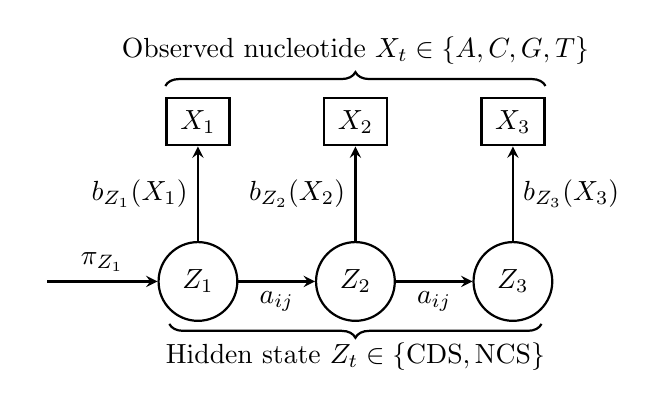
\begin{tikzpicture}[
    node distance=2cm,
    >=stealth,
    thick,
    state/.style={circle,draw,minimum size=10mm},
    obs/.style={rectangle,draw,minimum width=8mm,minimum height=6mm}
]

% Hidden states
\node[state] (z1) {$Z_1$};
\node[state,right of=z1] (z2) {$Z_2$};
\node[state,right of=z2] (z3) {$Z_3$};

% Observations
\node[obs,above=1.2cm of z1] (x1) {$X_1$};
\node[obs,above=1.2cm of z2] (x2) {$X_2$};
\node[obs,above=1.2cm of z3] (x3) {$X_3$};

% Transitions between hidden states
\draw[->] (z1) -- (z2) node[midway,below] {$a_{ij}$};
\draw[->] (z2) -- (z3) node[midway,below] {$a_{ij}$};

% Emissions
\draw[->] (z1) -- (x1) node[midway,left] {$b_{Z_1}(X_1)$};
\draw[->] (z2) -- (x2) node[midway,left] {$b_{Z_2}(X_2)$};
\draw[->] (z3) -- (x3) node[midway,right] {$b_{Z_3}(X_3)$};

% Initial distribution
\node[left=1.4cm of z1] (start) {};
\draw[->] (start) -- (z1) node[midway,above] {$\pi_{Z_1}$};

% Braces / annotations
\draw [decorate,decoration={brace,amplitude=5pt,raise=5pt,mirror}]
  (z1.south west) -- (z3.south east)
  node[midway,below=8pt] {Hidden state $Z_t \in \{\text{CDS}, \text{NCS}\}$};

\draw [decorate,decoration={brace,amplitude=5pt,raise=4pt}]
  (x1.north west) -- (x3.north east)
  node[midway,above=8pt] {Observed nucleotide $X_t \in \{A,C,G,T\}$};

\end{tikzpicture}
\vspace{-10pt}
\end{wrapfigure}
We develop a Hidden Markov Model (HMM) that accurately classifies a DNA sequence as a CDS or NCS. We apply an HMM because it reflects DNA structure well, since it contains a sequence of nucleotide observations ($X_t \in$ \{Adenine (A), Guanine (G), Cytosine (C), Thymine (T)\}) which have unique functions, reflected by the hidden states ($Z_t$). The structure of the observations are 3-mer sequences of nucleotides, $X_t,X_{t+1},X_{t+2}$, such as ACG or TGA. We follow the following conditional independence structure: \\
\[
P(Z_1) = \pi_{Z_1}, \qquad
P(Z_t \mid Z_{1:t-1}) = P(Z_t \mid Z_{t-1}) = a_{Z_{t-1},Z_t},
\]
\[
P(X_t \mid Z_{1:t}, X_{1:t-1}) = P(X_t \mid Z_t) = b_{Z_t}(X_t),
\]
As shown above, the hidden state is initialized from a distribution, $\pi$. The transition and emission matrices are derived from the conditional independence relationship and are parametrized as $a_{Z_{t-1},Z_t}$ and $b_{Z_t}(X_t)$.
\subsection{Inference/Learning Algorithm}
Since our dataset is fully labeled with the true CDS/NCS state for each 3-mer,
we train the HMM in a supervised manner. We use the
\texttt{hmmlearn} library to compute maximum likelihood estimates of the
initial distribution $\pi$, the transition matrix $A$, and the emission matrix
$B$ from empirical counts in the training set.

During evaluation on the test genome sequence, the true labels are hidden and
must be inferred. We apply the Viterbi algorithm to compute the most probable
sequence of hidden states $Z_{1:T}$ given the observed 3-mer sequence
$X_{1:T}$. This allows us to compare the predicted CDS/NCS hidden state
against the ground-truth genome annotation and measure model accuracy.

\subsection{Simplifications and Assumptions}
Note that as a simplification, we assume each nucleotide is independent and identically distributed. This is not necessarily always true in reality, because certain parts of DNA sequences may have varying ratios of nucleotides (e.g. sequences whose GC content is higher.) But for this model, the IID assumption is not too large a leap in logic, and thus it will be applied to allow the application of a HMM.

\section{Results and Discussion}

Currently, we trained our preliminary HMM on the
Saccharomyces cerevisiae 3-mer dataset described in Section 2.1.
Each of our observations can be one of the 64 possible nucleotide 3-mers, with
corresponding hidden states as CDS or NDS which indicate
whether the central base in the 3-mer lies inside a coding region or a
noncoding region according to the GFF annotation.

Using the hmmlearn library, we instantiated a two-state CategoricalHmm, that consists of 64 discrete emission categories corresponding
to all possible 3-mers. We fit the model on the full yeast genome 3-mer
sequence, decoding the most likely hidden-state sequence with the
Viterbi algorithm. For our first sanity check, we compared predicted
hidden-state labels against the ground-truth CDS and NCS labels from the
annotation. This yielded an overall accuracy of around
\(\mathbf{45\%}\) on the 3-mer sequence.
(In the current version, we 
evaluate on the same data used for fitting but in future work we plan on introducing a
proper train/test split.)

While \(45\%\) accuracy shows that the model is still learning, it's
still far from our expectations so we're working towards improving it. Some reasons why our model performed this way could be the following:
\begin{itemize}
    \item \textbf{No explicit supervision in fitting:} Since we're using the default EM procedure in hmmlearn, which treats
      the CDS/NCS state as latent during learning, the hidden states are
      then aligned to the CDS and NCS labels only post hoc when computing
      accuracy. This means that the model is not yet fully using the fact that
      we have labeled training data.
    \item \textbf{Class imbalance and simple structure:} Since the yeast genome
      contains long stretches of noncoding sequence, this could mean that a trivial baseline that
      always predicts ``noncoding'' can already achieve non-trivial accuracy.
      Also, our current HMM only has two states and since we assume i.i.d.\ emissions given
      the state, we assume it cannot yet capture richer patterns such as different
      statistics in start/stop codons or UTR regions.
    \item \textbf{Lack of proper evaluation protocol:} Since we currently train and
      evaluate on the same 3-mer sequence this can inflate performance and
      will not accurately reflect generalization to unseen genomic regions.
\end{itemize}

Despite this, our first draft confirms that the overall pipeline
is functioning end-to-end. We can, (1), parse an annotated genome into labeled
3-mers, (2), fit a two-state HMM with discrete emissions, and (3), run
Viterbi decoding to obtain a CDS/NCS segmentation that can be compared
quantitatively to the annotation. This allows for a clear path for more careful
experiments in the next milestone.

\subsection*{Planned Improvements}

To improve, we have some ideas:
\begin{itemize}
    \item Switching from unsupervised EM fitting to a supervised or
      semi-supervised estimation using the labeled CDS/NCS
      sequence to compute maximum-likelihood estimates of \(\pi\), \(A\), and
      \(B\).
    \item Introduce a proper train/validation/test split over the genome (such as holding out contiguous chromosomal segments) so that we can avoid overfitting to a single sequence and evaluate generalization.
    \item Compare against simple baselines like majority-class predictor,
      a logistic-regression classifier on 3-mer counts, or a Markov chain over
      nucleotides without hidden states.
    \item Explore richer state spaces (separating introns, exons, and
      UTRs) or switch between observation choices (longer k-mers) to see
      whether the HMM can better reflect biologically meaningful patterns in genome.
\end{itemize}

\section{Conclusion}

In this project we created a probabilistic modeling of coding
versus noncoding regions in eukaryotic genomes using HMMs. We
constructed a labeled dataset of overlapping 3-mers from the
S.cerevisiae reference genome and implemented an HMM whose two hidden
states correspond to CDS and NCS. We used an hmmlearn based model,
trained on the yeast 3-mer sequence and decoded with Viterbi, achieving around
\(45\%\) accuracy when predicting CDS/NCS labels, which indicates that there is
signal in the 3-mer distribution.

Although the current results are limited and there is still room for improvement, the end-to-end pipeline from raw
FASTA/GFF files to genome parsing, HMM construction, and Viterbi
decoding gives us a solid starting area for fine tuning. By using supervised parameter
estimation, more principled evaluation, and potentially richer state spaces
and observation models, we aim to significantly improve CDS/NCS
classification performance and move closer to a biologically meaningful model
of eukaryotic gene structure.

\section{Reflections \& Contributions}
Upon further reflection, using a larger dataset and a wider variety of data across different species would be interesting further research. \\
For team contributions, Jared cleaned and setup the dataset and wrote problem description and data sourcing report sections. Tej setup the model, and trained/evaluated the HMM. Justin generated results/conclusion and wrote report for those sections. Conor setup the model/inference structure and wrote the report section about it as well as the reflections/contributions section. \\
Gen AI was used to assist in the creation of the LaTex diagrams/equations. 
 
%%%%%%%%%%%%%%%%%%%%%%%%%%%%%%%%%%%%%%%%%%%%%%%%%%%%%%%%%%%%

% \appendix

% \section{Appendix / supplemental material}


% Optionally include supplemental material (complete proofs, additional experiments and plots) in appendix.
% All such materials \textbf{SHOULD be included in the main submission.}

%%%%%%%%%%%%%%%%%%%%%%%%%%%%%%%%%%%%%%%%%%%%%%%%%%%%%%%%%%%%

\bibliographystyle{plainnat}
\bibliography{references}
\end{document}